\section{Design}
\label{sec:design}

\subsection{Secure Isolation}
The two primary goals of our design is to a. Provide isolation of selected applications on mobile phones and b. To build a usable solution which can be integrated seamlessly into the host operating system of the smartphone. To achieve these goals we either need a type-II hypervisor which can run within the host operating sysystem or employ OS-level virtualization techniques like containers.  Unlike conventional virtualization, containers have almost no overhead as they do not run the entire software stack of the guest operating system.  On the other hand, because the virtualization is facilitated by the operating system, other OSes or architectures cannot be used within a container.In our design, we propose to use operating system level virtualization techniques of which Linux Containers and OpenVZ are popular implementations.\\
\Comment{Need a couple of references here to OpenVZ: \cite{OpenVZ} and LSM: \cite{LSM}}
 
\subsection{Linux Containers}
Linux Containers (LXC) implement OS-level virtualization techniques in order to run a number of isolated virtual environments on a single host.  LXC differs from conventional virtualization techniques, which generally require the installation of guest OSes.  The isolated virtual environments or containers, are built upon other Linux security mechanisms. We list the different resources isolated using containers and the techniques used for them below.
% such as   runs processes on a Linux kernel, other OSes such as Windows and other UNIXes (BSD or OSX) can not be used as containers.  

%To achieve the first goal, we propose to use 
\Comment{Someone should finish this}
%first investigated Type-II virtualization techniques which allow a guest operating system to run from within the host operating system.

\begin{figure}[tbh]
\centering
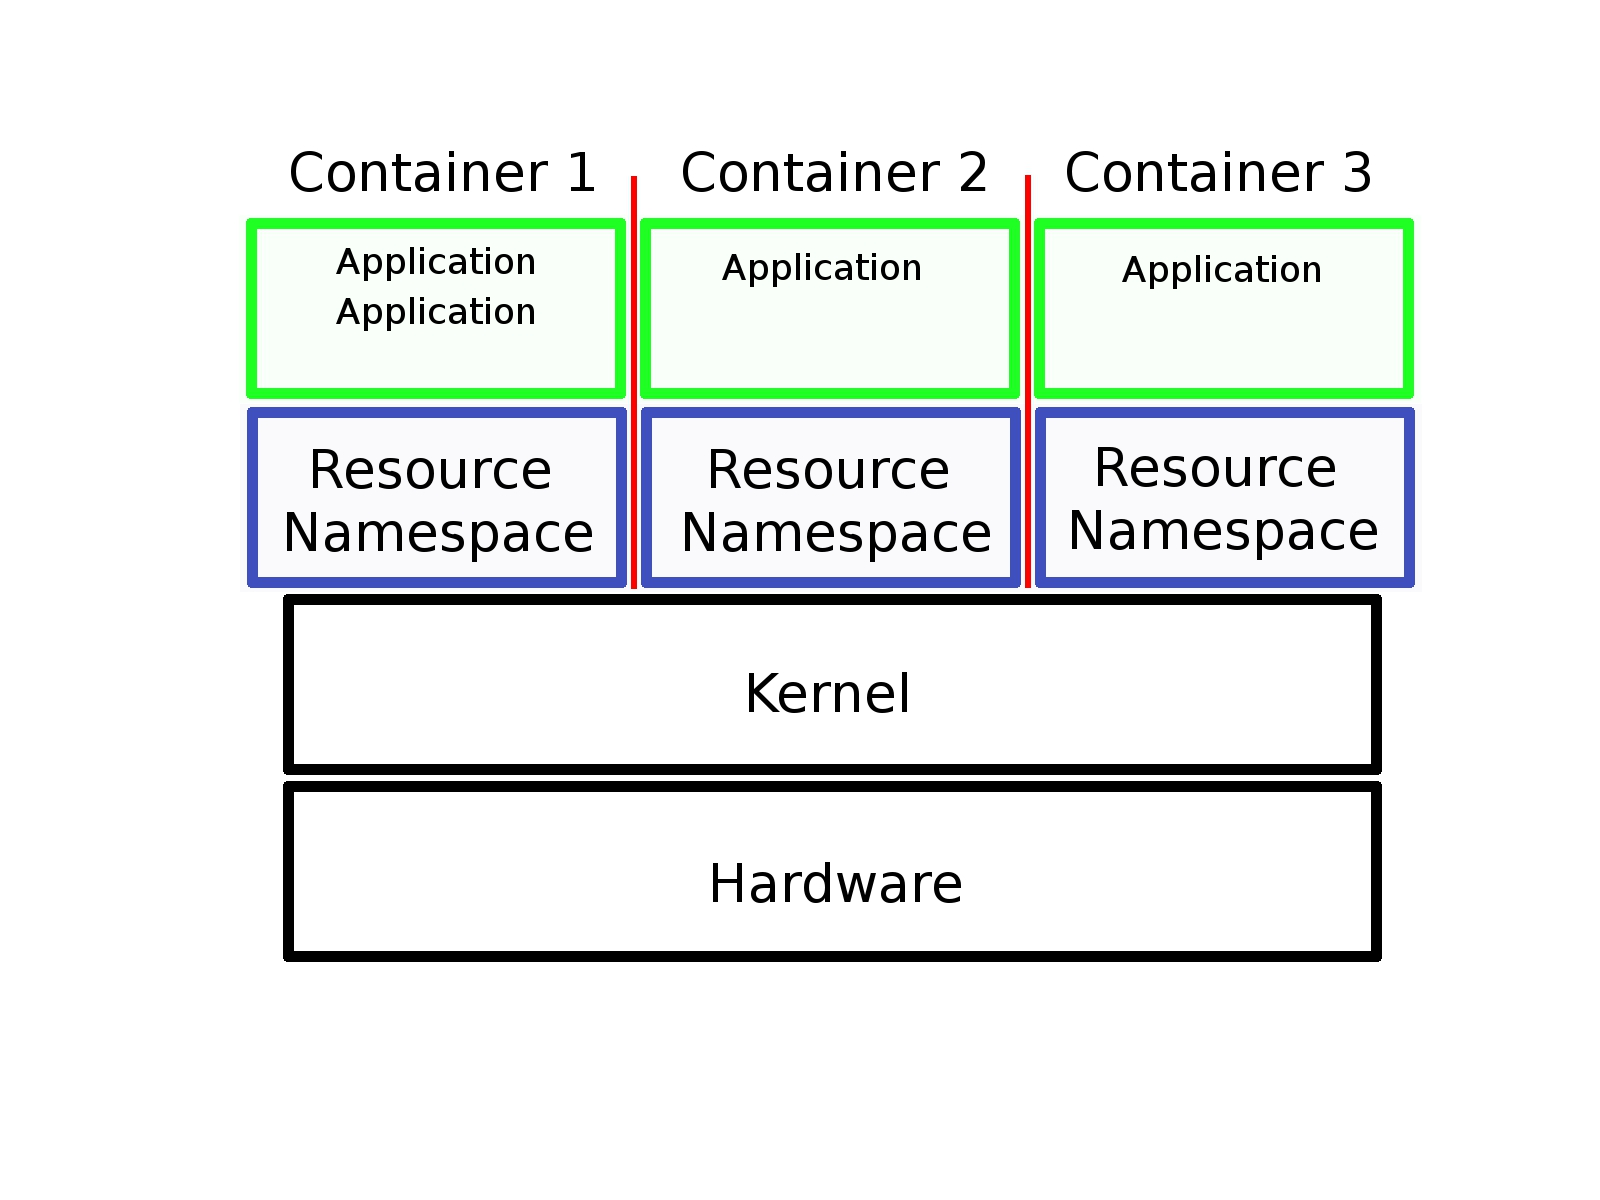
\includegraphics[width=1.0\columnwidth]{containers}
\caption{Linux Container Architecture}
\label{fig:containers}
\end{figure}


\subsection{Host Identification}
On Linux machines, the identity of a system is usually established through the command `uname'. This command reads informations stored in the structure `utsname'. The structure includes the name of the operating system in use and the current version of the operating system. The structure also contains the hostname of the machine and this is used to identify the machine in network communications. Linux Containers implement a per-process utsname namespace and this enables each container to have a different hostname.

\subsection{Process Identifiers}
Process identifiers (PIDs) are isolated using PID namespaces such that with respect to each container the set of PIDs appears like a standalone machine. This also allows two processes to  have the same PID in different containers. Processes can be launched in a new PID namespace using the clone or the unshare system-calls. This is an important feature for enabling migration of containers between hosts as the same PID values can be maintained at the source and destination. Also, PID namespaces are hierarchical; tasks in the original namespace can see the PIDs of tasks in the new namespace but not vice-versa.  

\subsection{Inter-Process Communications}
Inter-Process Communication (IPC) between processes uses shared objects like shared memory segments, message queues etc. To create isolated environments, it is necessary that processes from one container cannot share data or communicate with other containers. This is achieved by introducing IPC namespaces which creates separate set of IPC objects for each container.

\subsection{User Namespaces}
Utsname namespaces were first available in Linux kernel 2.6.19.  Utsname supplies information about a system's hostname.  With Utsname, different processes can be associated with different hostnames, and jobs being migrated can take their hostnames with them.

\subsection{Network Devices}
The Linux kernel 2.6.26 was the first version to include network namespaces.  The network namespaces assigns a private set of network resources, including IP addresses, routes, sockets, and more, to any number of processes.  This allows for shared names among different namespaces and isolation between those namespaces.  This provides substantial improvements in security, network resource management, namespace consolidation, and mobility.

\subsection{Readonly-bind mounts}
Readonly-bind mounts have been available since Linux kernel 2.6.24.  This allows for read-only accesses to a filesystem mounted read-write.  It guarantees that one process can read and write to the filesystem, while others can only write to it, regardless of their privileges.

\subsubsection{Copy-on-Write filesystems}

Resource namespaces allow containers to manipulate the accessing of processes, files, and hardware resources.  Control groups are used to limit the resources used by a container.  Capability bounding sets reduce a container's privileges.  

The main obstacle to using Linux Containers are the requirements.  LXC requires a Linux kernel version 2.6.27 or greater, and the Pre is running 2.6.24.  The kernel functionality would have to be back ported in order to work with the Pre.  The Android is running 2.6.29; however, porting the LXC tools to Android will likely be very difficult.
